\clearpage
\section{Statistical Analysis}
With a large dataset, previous "event display" method will no longer be efficient and accurate. Thus data analysis tools are necessary. Here \verb|root| is used and three macros to apply cuts are already implemented. As before we have four sets of Monte Carlo simulated data in order to find the optimal cuts, then there are a couple of real data samples.

For some reason, variables in \verb|root| files unfortunately have different names. Here we have the same four variable and an addition parameter~\cite{manual}
\begin{itemize}
	\item \verb|Ncharged|: number of charged tracks (\verb|Ctrk(N)|)
	\item \verb|Pcharged|: total scalar sum of track momenta (\verb|Ctrk(SumP)|)
	\item \verb|E_ecal|: total energy in electromagnetic calorimeter (\verb|Ecal(SumE)|)
	\item \verb|E_hcal|: total energy in hadronic calorimeter (\verb|Hcal(SumE)|)
	\item \verb|cos_thet|: cos(polar angle) between incoming positron and outgoing positive particle
\end{itemize}

\subsection{Mode selection}
\begin{figure}[ht]
	\centering
	\includegraphics[width=0.8\linewidth]{cos_thet_before.pdf}
	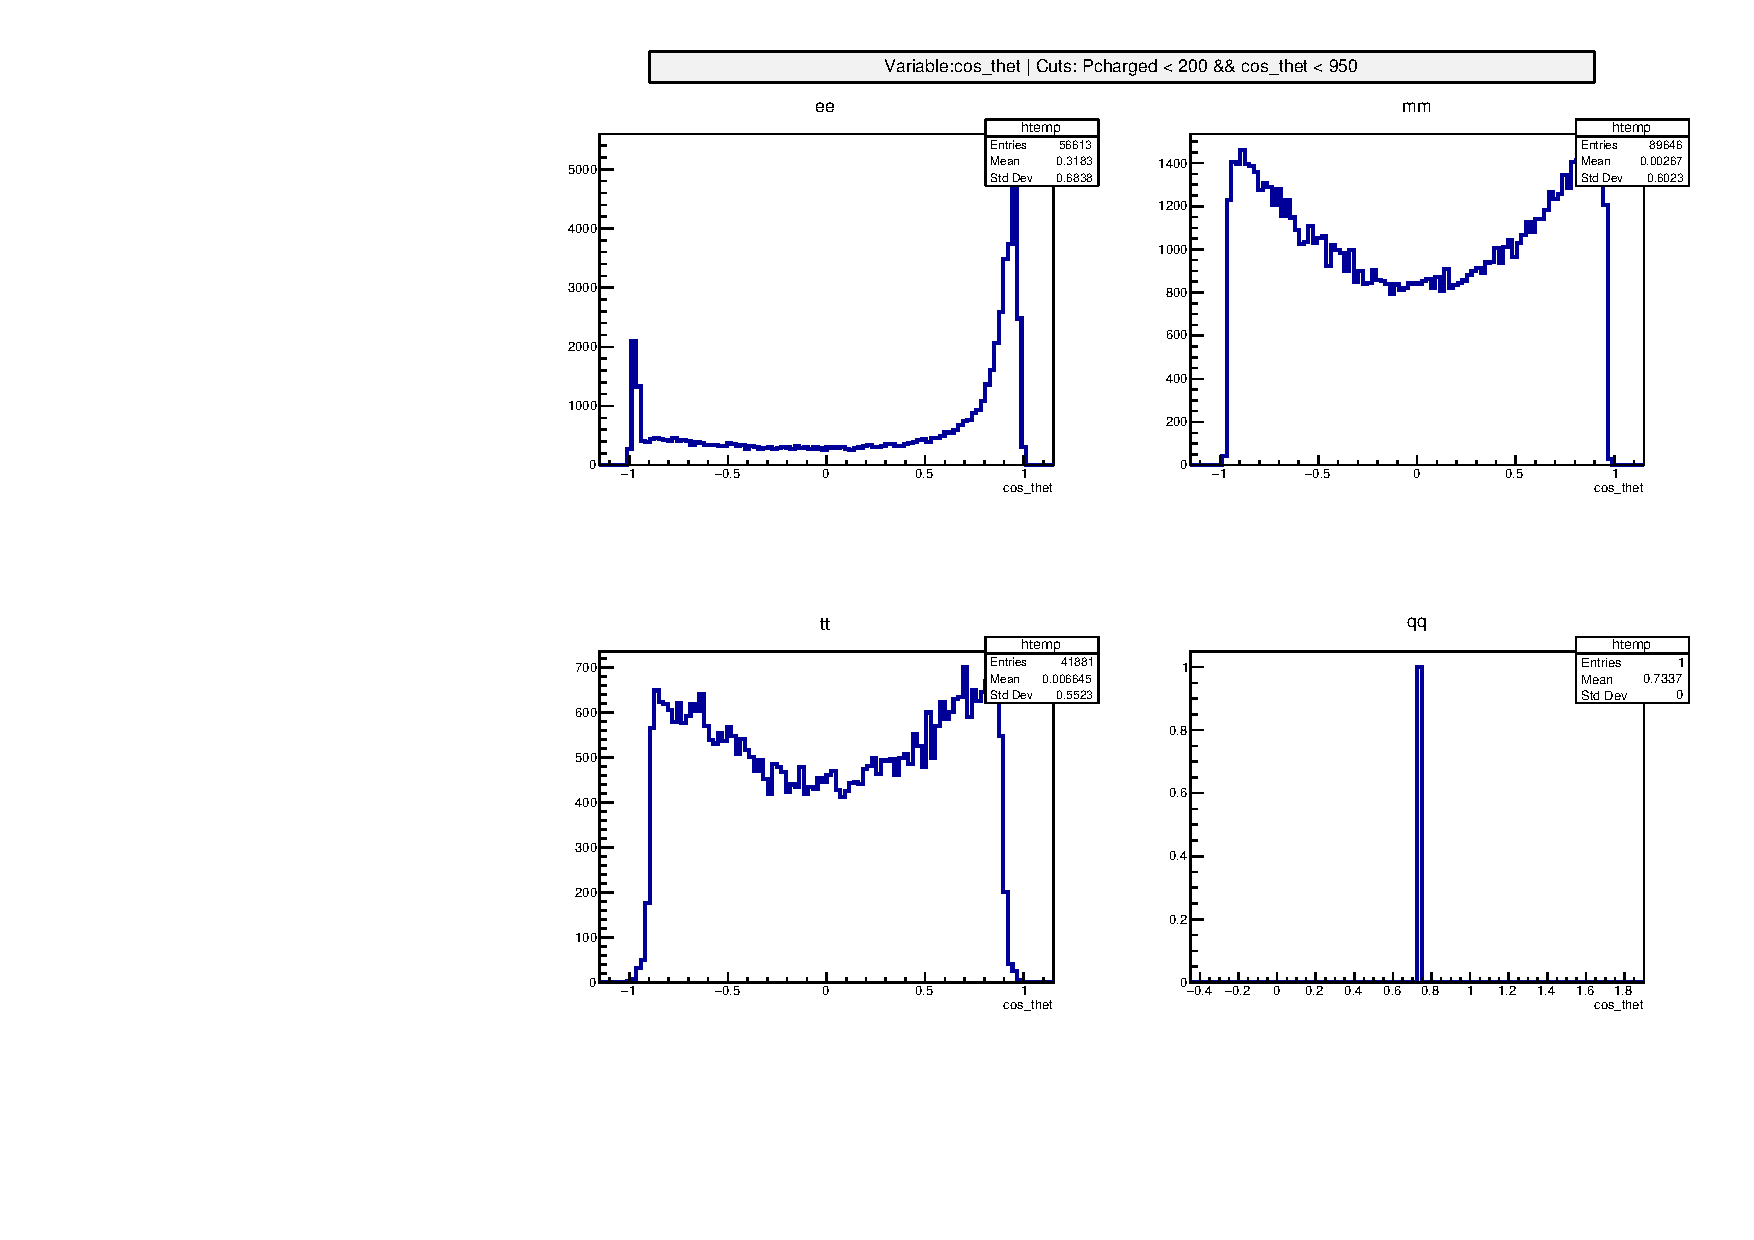
\includegraphics[width=0.8\linewidth]{cos_thet_after.pdf}
	\cprotect\caption{Distribution of \verb|cos_thet| before and after \verb|cos_thet| cut.}%
	\label{fig:cos_thet_cut}
\end{figure}
First of all, there are a couple of general cuts. The collider energy of LEP is $\sim\SI{200}{\giga\eV}$. Thus the scalar sum of momenta should be maximally around this value. Events with even larger momenta are caused by various unphysical processes. Secondly, the data here is written such as when there are multiple outgoing positive particles, $\verb|cos_thet|=1000$. For $ee$ and $\mu\mu$ process, it should not be possible, since no hadronisation can occur and initial/final state radiation for these two only involve photons. So for these two event selections, cut $\verb|cos_thet| <= 1.0$ is applied, see figure~\ref{fig:cos_thet_cut}. After the cut(s), there are $56613$ $ee$ events, $89646$ $\mu\mu$ events, $79099$ $\tau\tau$ events, and $98100$ $qq$ events.

In event display part, we have success using cut $\verb|Ncharged| > 7$ for $qq$ processes. We conclude that this is no longer sufficient, since there are quite many $\tau\tau$ contamination, see figure~\ref{fig:qq_Ncharged_cuts}. While roughly $5\%$ percent of $qq$ events are lost, $\tau\tau$ events are barely present and $ee$, $\mu\mu$ are completely cut. So the $5\%$ percent are considered as acceptable "casualties". We drop the cut in \verb|E_ecal|. After the cut for $qq$, no $ee$ or $\mu\mu$ are left, $78$ $\tau\tau$ survives and $92688$ $qq$ events remain.
\begin{figure}[ht]
	\centering
	\includegraphics[width=0.8\linewidth]{N_charged_before2.pdf}
	\includegraphics[width=0.8\linewidth]{N_charged_after.pdf}
	\cprotect\caption{Number of charged tracks (\verb|Ncharge|) before and after the refined cut for $qq$ events.}%
	\label{fig:qq_Ncharged_cuts}
\end{figure}

Follow the same receipt as in event display part, we try to separate $ee$ events from other leptonic channels. Cut in number of charged track remains the same: $\verb|Ncharged| < 4 $ or ($\leq 3$). Same as before \verb|E_ecal| of $ee$ events have peak at around \SI{80}{\giga\eV}. \verb|E_ecal| cut is changed to $\verb|E_ecal| > 60$, since there is virtually no events even at $\verb|E_ecal| = 60$, see figure~\ref{fig:ee_cuts}. \verb|E_hcal| cut is similar to before, just relaxed a little bit (to \verb|E_hcal < 2|), since some of events have higher \verb|E_hcal| as previous cut, see figure~\ref{fig:ee_cuts_hcal}. In the end, we end up with $51679$ $ee$ events, $0$ $\mu\mu$, $910$ $\tau\tau$ events, and $1$ $qq$ event.
\begin{figure}[ht]
	\centering
	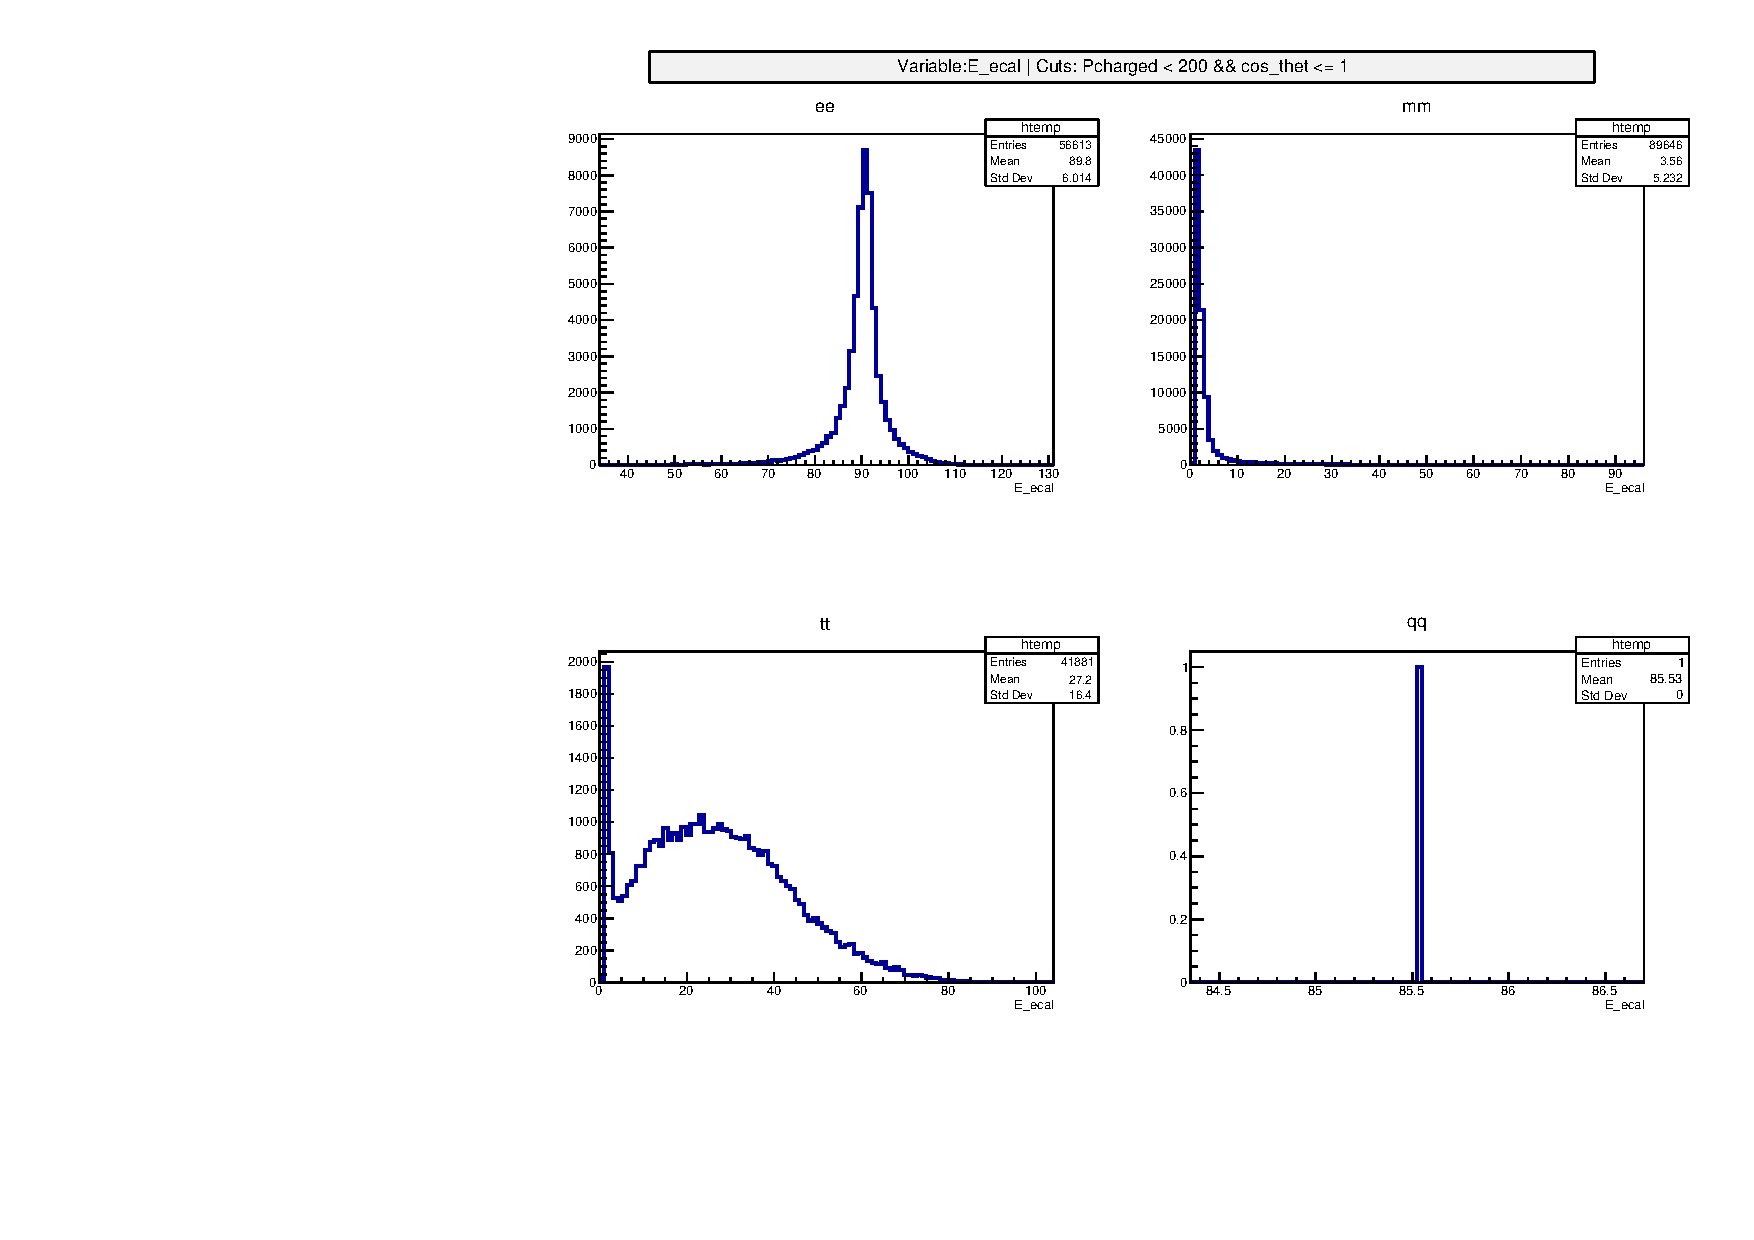
\includegraphics[width=0.8\linewidth]{ecal_before_ecal_cut.pdf}
	\cprotect\caption{\verb|E_ecal| distribution before \verb|E_ecal| cut for $ee$. }%
	\label{fig:ee_cuts}
\end{figure}
\begin{figure}[ht]
	\centering
	\includegraphics[width=0.8\linewidth]{hcal_after_Ncharged_ecal_cuts.pdf}
	\cprotect\caption{\verb|E_hcal| distribution after \verb|E_ecal| but before \verb|E_hcal| cut for $ee$.}%
	\label{fig:ee_cuts_hcal}
\end{figure}


For $\mu\mu$ selection, cut in \verb|Ncharged| is the same as $ee$: $\verb|Ncharged|< 4$. We have already seen in figure~\ref{fig:ee_cuts} that \verb|E_ecal| of $\mu\mu$ has a peak around $0$, so the \verb|E_ecal| cut for $ee$ gets inverted as cut for $\mu\mu$: $\verb|E_ecal| < 60$. Then remaining $\tau\tau$ events can be excluded with the help of \verb|Pcharged|, see figure~\ref{fig:mm_cuts}. $ee$ and $qq$ events are basically cut away, only unwanted events are $\tau\tau$. \verb|Pcharged| distributions of $\mu\mu$ and $\tau\tau$ are separated quite nicely, although some $\mu\mu$ events have $\verb|Pcharged| \approx 0$. A cut at $\verb|Pcharged| > 70$ will remove most of $\tau\tau$ events while preserve most of $\mu\mu$ events. After combinations of these cuts, $144$ $ee$ events, $83228$ $\mu\mu$ events, $480$ $\tau\tau$ events and zero $qq$ event survive.
\begin{figure}[ht]
	\centering
	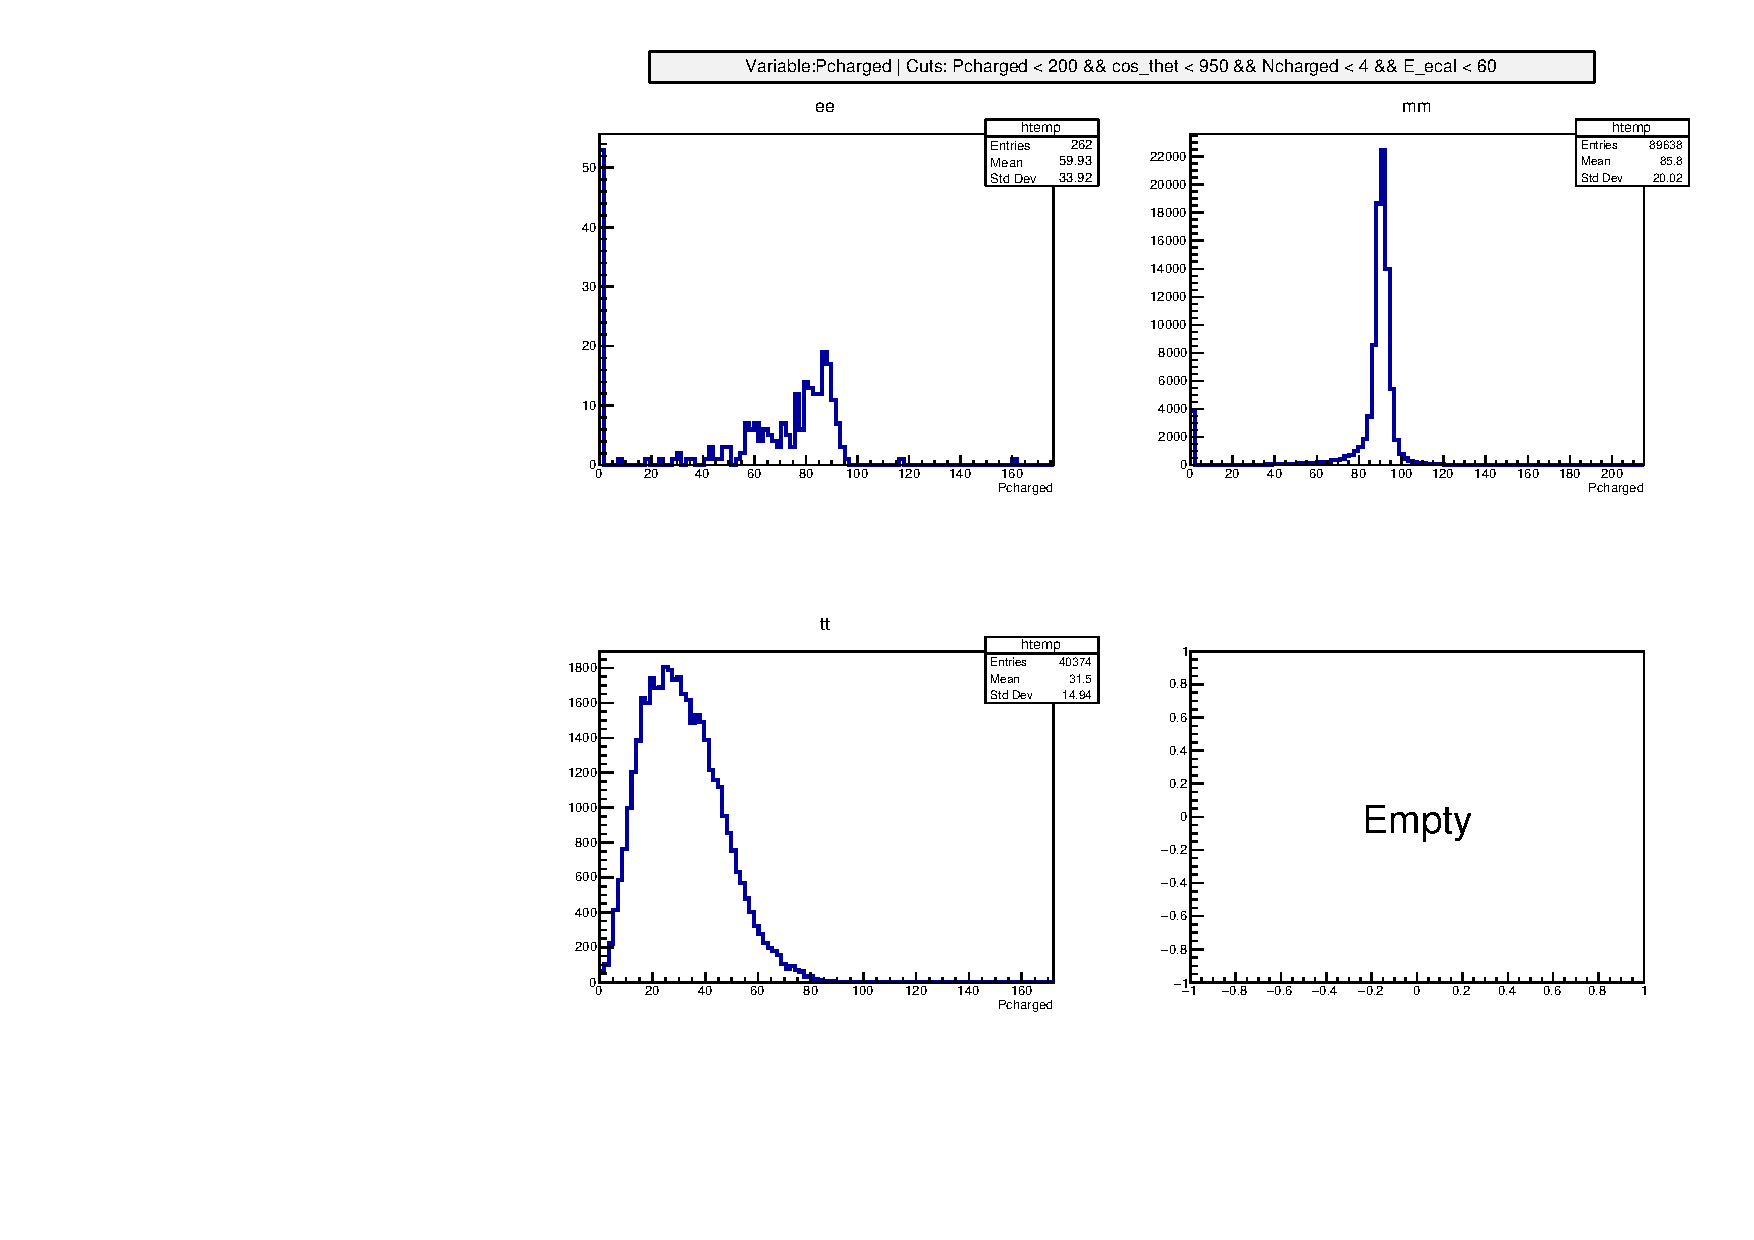
\includegraphics[width=0.8\linewidth]{Pcharged_mm_before_pcharged_cut.pdf}
	\cprotect\caption{\verb|Pcharged| distribution after \verb|E_ecal| cut for $\mu\mu$.}%
	\label{fig:mm_cuts}
\end{figure}

$\tau\tau$ can be picked out using the same cuts for $\mu\mu$ expect $\verb|Pcharged|$ cut gets inverted. Since there is a small peak at $\verb|Pcharged| = 0$ in $ee$ and $\mu\mu$ events, see figure~\ref{fig:mm_cuts}, a lower bound in \verb|Pcharged| should be set as well. Thus for $\mu\mu$: $1< \verb|Pcharged| < 60$. $E_ecal$ cut should be adjusted a bit. In figure~\ref{fig:ee_cuts}, there are still quite substantial amount of $\tau\tau$ event between $60 < \verb|E_ecal| < 70$. Thus we have for $\tau\tau$: $\verb|E_ecal| < 70$. Cut in \verb|Ncharged| is relaxed to $<5$ for better efficiency. After all these cuts, we have $243$ $ee$ events, $1446$ $\mu\mu$ events, $66990$ $\tau\tau$ events, and $38$ $qq$ events.

All the cuts are summarizes in table~\ref{tab:cuts_all}
\begin{table}[ht]
	\centering
	\begin{tabular}{cccccc}
		\toprule
	mode & \verb|cos_thet| & \verb|Pcharged| & \verb|Ncharged| & \verb|E_ecal| & \verb|E_hcal| \\
	\midrule
	$ee$ & $\leq 1$ & $< 200$ & $< 4$ & $>60$ & $< 2$ \\
	$\mu\mu$ & $\leq 1$ & $>70, <200$ & $<4$ & $<60$ & \\
	$\tau\tau$ & & $>1, <60$ & $<5$ & $<70$ \\
	$qq$ & & $<200$ & $>10$ & & \\
	\bottomrule
	\end{tabular}
	\caption{All cuts applied to select decay modes}
	\label{tab:cuts_all}
\end{table}

\clearpage
\subsection{Channel selection} Since processes with $e^+ e^-$ as final states include also $t$-channel elastic scattering between electron and positron and they are irrelevant processes in our discussion, we want to somehow get rid of these contributions. From figure~\ref{fig:angDep} in pre-lab tasks, we know that $s$-channel dominates at small $\cos\Theta$ and $s$-channel contributions should look like symmetric around $\cos\Theta = 0$. Naturally, first thing comes in our minds is to cut $\cos\Theta$ from somewhere between $0$ and $1$ to $-\infty$, so that it looks symmetric. Figure~\ref{fig:s_t_cut} is done with $\cos\Theta < 0.5$. There is a quite significant peak around $\cos\Theta = -1$, which we don't really expect. Physical origin of this peak is unknown to us, but anyway this should be cut away. In the end, we have the cut $-0.9 < \cos\Theta < 0.5$. This cut along with the previous $ee$ cuts will be the new $ee$ cuts used onwards.
\begin{figure}[ht]
	\centering
	\includegraphics[width=0.8\linewidth]{s_t_cut.pdf}
	\caption{$\cos\Theta$ distribution of $ee$ events after previously determined $ee$ cuts and $\cos \Theta< 0.5$.}%
	\label{fig:s_t_cut}
\end{figure}

\subsection{Forward-backward asymmetry}
Numbers of events in forward ($0 <\cos\theta<1$) and backward ($-1<\cos\theta<0$) are measured using \verb|data1.root| and MC data with $\mm$ as final states. In the actual analysis, only the real data are used. Upon inspection of definition~\ref{math:AFBdef}, it is clear that correction for cut efficiency is unnecessary here, since $N_{+,-}$ share the same cuts.

After application of equation~\ref{math:AFBdef} at all available CMS energy, correction terms should be added to the measured asymmetry. As we understand it, applying these corrections will remove radiation corrections in measured data, so that we can directly compare experimental values with tree-level theoretical values.
\begin{figure}[ht]
	\centering
	\includegraphics[width=0.8\linewidth]{A_FB.pdf}
	\caption{Forward-backward asymmetry after applying corrections. }%
	\label{fig:A_FB}
\end{figure}

Figure~\ref{fig:A_FB} shows the forward-backward asymmetry at various CMS energies. Errors are calculated as usual $\sigma_N \approx \sqrt{N}$.

If one says that the fourth data point (with $\sqrt{s} =\SI{91.22}{\giga\eV}$) lies \textit{exactly} at the peak of resonance, this $A_\text{FB}$ can be used to determined the Weinberg angle from equation~\ref{math:AFBpeak}
\begin{align*}
	\sin^2\theta_W &= \frac{1-\sqrt{A^{\mu, \text{peak}}_{\text{FB}}/3}}{4} \\
	\sigma_{\sin^2\theta_W} &= \frac{1}{8\sqrt{3}} \frac{\sigma_A}{\sqrt{A}}	
\end{align*}
Then we have
\begin{equation}
	\sin^2\theta_W = \num{0.2347 +- 0.0112}
\end{equation}

From PDG~\cite{PDG}, in $\bar{\text{MS}}$ and $\sqrt{s} = M_Z$, the angle is $\sin^2\theta_W = \num{0.23121 +- 0.00004}$. Our value matches it quite well.

In principle one can calculate the Weinberg angle at every CMS energy using equation~\ref{math:AFBgen}. But then according to QFT, value of Weinberg angle also changes, since it depends on the coupling $g$ and $g'$. Thus we just settle with this value as our final result.

\subsection{Cut efficiency}
Cut efficiency can be defined as
\begin{equation}
	\epsilon_{ij} = \frac{N_i}{N_j}
\end{equation}
where a cut $i$ is applied to a process $j$. In previous sections, there are multiple cuts and MC simulation data. By applying all the cuts to all the data, a $4\times4$ efficiency matrix can be obtained
\begin{align}
	\mathbf{\epsilon} &= \begin{pmatrix} N_{ee, \text{cuts}}/N_{ee} & N_{ee, \text{cuts}}/N_{\mm} & N_{ee, \text{cuts}}/N_{\tta} & N_{ee, \text{cuts}}/N_{qq} \\ 
	N_{\mm, \text{cuts}}/N_{ee} & N_{\mm, \text{cuts}}/N_{\mm} & N_{\mm, \text{cuts}}/N_{\tta} & N_{\mm, \text{cuts}}/N_{qq} \\ 
	N_{\tta, \text{cuts}}/N_{ee} & N_{\tta, \text{cuts}}/N_{\mm} & N_{\tta, \text{cuts}}/N_{\tta}  &N_{\tta, \text{cuts}}/N_{qq} \\ 
	N_{qq, \text{cuts}}/N_{ee} & N_{qq, \text{cuts}}/N_{\mm} & N_{qq, \text{cuts}}/N_{\tta}  &N_{qq, \text{cuts}}/N_{qq} 
\end{pmatrix} \label{math:epsFor}\\
							&= \begin{pmatrix} \num{0.9667 +- 0.0096} & \num{0.0000 +- 0.0000} & \num{0.0082 +- 0.0003} & \num{0.0000 +- 0.0000} \\ 
								\num{0.0070 +- 0.0006} & \num{0.9284 +- 0.0045} & \num{0.0061 +- 0.0003} & \num{0.0000 +- 0.0000} \\
								\num{0.0153 +- 0.0009} & \num{0.0317 +- 0.0006} & \num{0.8881 +- 0.0046} & \num{0.0004 +- 0.0001} \\
								\num{0.0000 +- 0.0000} & \num{0.0000 +- 0.0000} & \num{0.0010 +- 0.0001} & \num{0.9448 +- 0.0043} 
	\end{pmatrix}\notag
\end{align}
Raw data can be found in appenfix~\ref{app:59}. Note that the total number of events considered here is the number \textit{after} the general \verb|Pcharged| and \verb|cos_thet| (including $s$-channel selection) cuts. After all, cuts efficiencies we discuss here are only the efficiencies of cuts like $ee$ cuts and so on.

Error is estimated using Poisson statistic and usual error propagation formula
\begin{equation*}
	\sigma_{\epsilon_{ij}} = \sqrt{ \left(\frac{1}{N_j} \sigma_{N_i} \right)^2 + \left(\frac{N_i}{N_j^2} \sigma_{N_j}\right)^2  }  = \sqrt{ \frac{N_i}{N_j^2} + \frac{N_i^2}{N_j^3} }
\end{equation*}

Actually the $\epsilon_{i, ee}$ efficiencies are problematic, because in \verb|cos_thet| cuts, one part of $s$-channel gets lost. Main purpose of efficiency matrix is to obtain true number of events from measured number of events. If we continue to use $\epsilon_{i, ee}$ without further corrections, the true number of events are of $-0.9 < \verb|cos_thet| < 0.5$, resulting lower counts. 

The correction involves adjustment of denominator or $\epsilon_{i, ee}$, since in selecting $N_{ee}$ the $s$-channel cuts are applied. For this, the function $(1+\cos^2\Theta)$ is integrated in $-0.9 < \cos\Theta < 0.5 $  and in $-1 < \cos\Theta < 1$.
\begin{equation}
	\text{corr. factor} = \frac{\int_{-1}^{1} \dd{x} (1+x^2)}{ \int_{-0.9}^{0.5}\dd{x} (1+x^2)} \approx \num{1.583}
\end{equation}
This number is then multiplied to all the denominator of first column in equation~\ref{math:epsFor}. Now the corrected efficiency matrix is
\begin{equation}
	\epsilon = \begin{pmatrix} \num{0.6107 +- 0.0061} & \num{0.0000 +- 0.0000} & \num{0.0082 +- 0.0003} & \num{0.0000 +- 0.0000} \\ 
								\num{0.0044 +- 0.0004} & \num{0.9284 +- 0.0045} & \num{0.0061 +- 0.0003} & \num{0.0000 +- 0.0000} \\
								\num{0.0097 +- 0.0006} & \num{0.0317 +- 0.0006} & \num{0.8881 +- 0.0046} & \num{0.0004 +- 0.0001} \\
								\num{0.0000 +- 0.0000} & \num{0.0000 +- 0.0000} & \num{0.0010 +- 0.0001} & \num{0.9448 +- 0.0043} 
	\end{pmatrix}
\end{equation}
This efficiency matrix is almost diagonal, which is expected if everything works fine.


\subsection{Partial cross sections}
From last section, cut efficiency matrix is obtained. It describes how true numbers of events $T_i$ translate into measured numbers of events $M_i$, i.e.
\begin{equation}
	\mathbf{M} = \epsilon \mathbf{T}
\end{equation}
In this compact matrix notation, $\mathbf{M}$ and $\mathbf{T}$ are vectors containing the numbers of events in a decay mode. Entries of $\mathbf{T}$ are listed in table~\ref{tab:510raw} in appendix.

With real data in \verb|data1.root|, we have the measured numbers using the cuts defined earlier. To find out true numbers, one needs to find inverse matrix $\epsilon^{-1}$.
\begin{equation}
	\mathbf{T} = \epsilon^{-1} \mathbf{M}
\end{equation}

We can propagate errors in $\epsilon$ and $\mathbf{M}$ to obtain an accurate error estimation of $\mathbf{T}$. According to~\cite{Lefebvre:400631},
\begin{equation}
	\text{Cov}(\epsilon^{-1}_{ab}, \epsilon^{-1}_{cd})= ([\epsilon^{-1}]_{a i} [\epsilon^{-1}]_{c i}) [\sigma_{\epsilon}]^2_{ij} ([\epsilon^{-1}]_{j b} [\epsilon^{-1}]_{j d})
\end{equation}
and the correlation matrix of $\mathbf{T}$ is
\begin{equation}
	\text{Cov}(T_i, T_j) = M_\alpha M_\beta \text{Cov} (\epsilon^{-1}_{i\alpha}, \epsilon^{-1}_{j\beta}) + \epsilon^{-1}_{ik} \epsilon^{-1}_{jl} \text{Cov}(M_k, M_l)
	\label{math:CovTT}
\end{equation}
where $\text{Cov}(M_k, M_l)$ is covariance matrix for measured counts and generally diagonal. This a bit complicated formula should be used instead of ignoring uncertainties in $\epsilon$. We have tested that simplification will lead to at least $50\%$ under-estimation of the errors.

After correction for efficiency, number of events needs to be divided by integrated luminosity $L = \int\dd{t} \mathcal{L}$ to obtain partial differential cross section (values listed in table~\ref{tab:lumi} in appendix). To account for higher order of Feynman diagrams, radiative corrections are added to the final results (see table~\ref{tab:rad_corr} in appendix). Determined partial cross sections are listed in table~\ref{tab:p_cross}
\begin{table}[ht]
	\centering
	\begin{tabular}{c cccc}
		\toprule
		$\sqrt{s}$ [\si{\giga\eV}] / $\sigma_i$[\si{\nano\barn}] & $ee$ &  $\mm$ &  $\tta$ & $qq$ \\ 
		\midrule 
		\num{88.47} & \num{0.389 +- 0.028} & \num{0.304 +- 0.018} & \num{0.338 +- 0.021} & \num{7.260 +- 0.094}\\
		\num{89.46} & \num{0.791 +- 0.043} & \num{0.656 +- 0.030} & \num{0.602 +- 0.030} & \num{14.105 +- 0.146}\\
		\num{90.22} & \num{1.221 +- 0.060} & \num{1.196 +- 0.047} & \num{0.980 +- 0.043} & \num{25.744 +- 0.230}\\
		\num{91.22} & \num{1.718 +- 0.032} & \num{1.805 +- 0.022} & \num{1.619 +- 0.022} & \num{40.578 +- 0.175}\\
		\num{91.97} & \num{1.094 +- 0.050} & \num{1.328 +- 0.044} & \num{1.107 +- 0.041} & \num{28.804 +- 0.231}\\
		\num{92.96} & \num{0.458 +- 0.041} & \num{0.562 +- 0.036} & \num{0.541 +- 0.037} & \num{13.721 +- 0.188}\\
		\num{93.71} & \num{0.323 +- 0.030} & \num{0.362 +- 0.025} & \num{0.308 +- 0.025} & \num{8.102 +- 0.125}\\
		\bottomrule
	\end{tabular}
	\caption{Partial cross section for various decay modes\label{tab:p_cross}}
\end{table}

Here the partial cross section is calculated with
\begin{equation}
	\pmb\sigma = \mathbf{L}^{-1} \mathbf{T}
\end{equation}
where $\pmb\sigma$ is vector like $\mathbf T$ and luminosity has been "promoted" to be a (diagonal) matrix $\mathbf L$. So formula~\ref{math:CovTT} can be used to calculate covariance matrix of partial cross sections. In table~\ref{tab:p_cross}, errors are propagated using only diagonal entries (variance) of the covariance matrix.

Figure~\ref{fig:lepCross} shows the partial cross sections of leptonic decay channels. Three curves are quite similar. From the numerical values in table~\ref{tab:p_cross}, one can see that the leptonic partial cross sections at peak ($\sqrt{s} = \SI{91.22}{\giga\eV}$) differ from each other at $\sim 2 \sigma$'s. Leptonic universality states that except mass difference, three generations of leptonic should behave the same. At such high energy ($\sqrt{s} \approx \SI{90}{\giga\eV}$), lepton masses are negligible and the partial cross sections should be identical. Here we do see some differences. This could be caused by some systematic regarding detection of one or more of the leptonic channels.
\begin{figure}[ht]
	\centering
	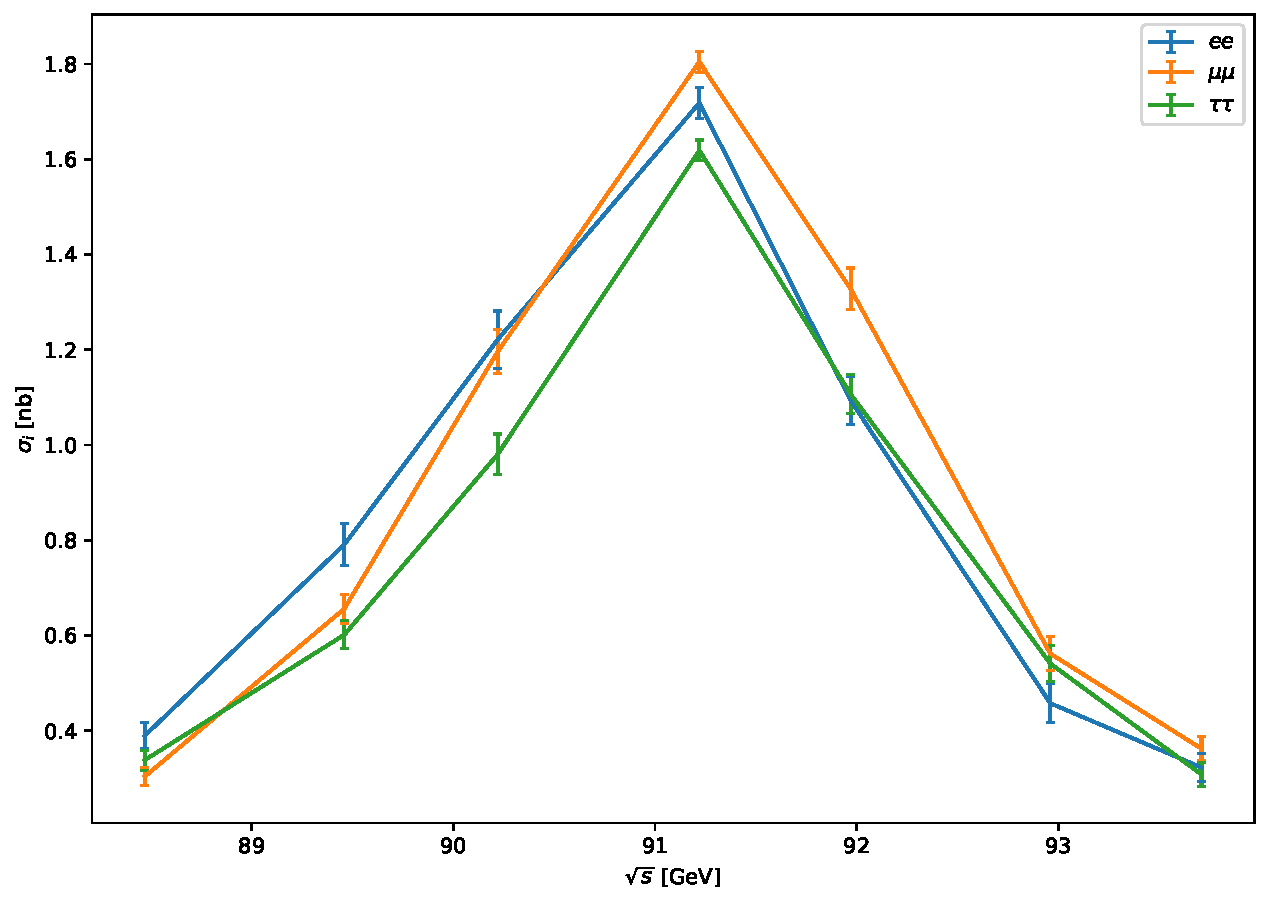
\includegraphics[width=0.7\linewidth]{sigma_lep.pdf}
	\caption{Partial cross section in leptonic channels}%
	\label{fig:lepCross}
\end{figure}

Partial cross sections to hadronic end states are quite high, because of the colour charge. Their partial cross sections are plotted in figure~\ref{fig:hadCross}.
\begin{figure}[ht]
	\centering
	\includegraphics[width=0.7\linewidth]{sigma_had.pdf}
	\caption{Partial cross section in hadronic channels}%
	\label{fig:hadCross}
\end{figure}

To compare theory and our measurement, one can try to calculate the ratios of hadronic cross section to (total) leptonic cross section. From the data, we have
\begin{equation}
	\left[ \frac{\sigma_\text{had}}{\sigma_\text{lep}} \right]_\text{exp}= \num{7.892 +- 0.076}
\end{equation}
whereas the theory predicts
\begin{equation}
	\left[ \frac{\sigma_\text{had}}{\sigma_\text{lep}} \right]_\text{theo}= \num{6.692}
\end{equation}
The measured value is quite off from the prediction, meaning it is not very likely that statistical fluctuations will explain this. A possible cause of this is the error could be underestimated somehow. Other factors like detection efficiencies and Monte Carlo simulation quality can play a role.

Actually this calculation can be misleading and inaccurate. With formula~\ref{math:CovTT}, we see that there should be correlation of different channels to some extent. But when calculating the ratio, this correlation is not considered. Instead, it would be better to draw $1\sigma$, $2\sigma$ etc. circles on $\sigma_\text{had}$-$\sigma_\text{lep}$ plane and see where the theoretical value lies. We reckon that it will not change the result too much and decide not to proceed with this method.

\subsection{Breit-Wigner fit}
For all decay modes, there is a clear peak at $\sqrt{s} = M_Z \approx \SI{91}{\giga\eV}$, where the partial cross sections increase drastically. This behaviour can be modelled with the Breit-Wigner form~\ref{math:sigmaf}, where $\Gamma_e$, $\Gamma_f$, $M_Z$ and $\Gamma_Z$ are the to be determined fit parameters. According to CERN documentation~\cite{cms}, the actual shape of curve might be a convolution of Breit-Wigner and Gaussian function, depending on the detector resolution. Here we will proceed with simple Breit-Wigner form.
\begin{figure}[ht]
	\centering
	\begin{subfigure}[b]{0.5\textwidth}
	\begin{center}
	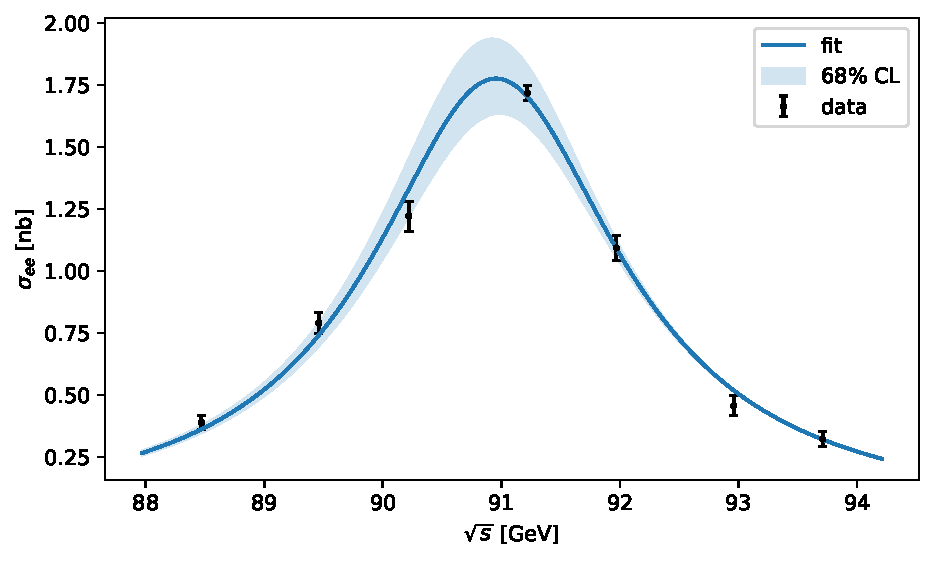
\includegraphics[width=\linewidth]{sigma_ee.pdf}%
	\end{center}
	\caption{$Z^0 \rightarrow ee$ partial cross section}
	\end{subfigure}%
	\begin{subfigure}[b]{0.5\textwidth}
	\begin{center}
	\includegraphics[width=\linewidth]{sigma_mm.pdf}
	\end{center}
	\caption{$Z^0 \rightarrow \mm$ partial cross section}
	\end{subfigure}
	\begin{subfigure}[b]{0.5\textwidth}
	\begin{center}
	\includegraphics[width=\linewidth]{sigma_tt.pdf}%
	\end{center}
	\caption{$Z^0 \rightarrow \tta$ partial cross section}
	\end{subfigure}%
	\begin{subfigure}[b]{0.5\textwidth}
	\begin{center}
	\includegraphics[width=\linewidth]{sigma_qq.pdf}
	\end{center}
	\caption{$Z^0 \rightarrow qq$ partial cross section}
	\end{subfigure}
	\caption{Partial cross section of all (visible) channels along with fit. Here the "$68\%$" CL regions are drawn only using the errors in $\Gamma_e$ and $M_Z$, since no errors in $\Gamma_e$ and $\Gamma_f$ can be reliably determined.}%
	\label{fig:p_cross_fit}
\end{figure}	

Since we have only $7$ data points but $4$ fit parameters for one channel, we should not expect the fit quality to be high (degrees of freedom $3$). (One can improve the fit by making $\Gamma_e \cdot \Gamma_f$ into a fit parameter, so that degrees of freedom decreases by $1$.) Actually, \verb|curve_fit| method in \verb|scipy| cannot give reliable estimation of covariance matrix involving $\Gamma_e$ and $\Gamma_f$. This can be caused by high condition number~\cite{stackoverflow}. This leads to a problem that errors of $\Gamma_e$ and $\Gamma_f$ cannot be provided in the fitting process. It should not be a big issue, since in this step we want to find out the $Z^0$ width and peak only. Also the errors in $\sigma_i$ are always from the diagonal entries of the covariance matrix, since the covariance matrices represent correlation of different cross sections at one certain CMS energy but here we plot one $\sigma_i$ at all CMS energies (otherwise one could input the appropriate covariance matrix into \verb|curve_fit|).

\begin{table}[ht]
\renewcommand{\arraystretch}{1.5}
	\centering
	\label{tab:label}
	\begin{tabular}{c | ccccc}
		\toprule
		channel & $\Gamma_e[\si{\mega\eV}]$ & $\Gamma_f[\si{\mega\eV}]$ & $\Gamma_Z[\si{\giga\eV}]$ & $M_Z[\si{\giga\eV}]$ & $\sigma_{i, \text{peak}}[\si{\nano\barn}]$\\
		\midrule 
		$ee$ & \num{84.568} & \num{77.060} & \num{2.551 +- 0.106} & \num{90.972 +- 0.033} & $1.777^{+0.159}_{-0.141}$\\
		$\mm$ & \num{84.209} & \num{77.171} & \num{2.513 +- 0.066} & \num{91.166 +- 0.029} & $1.818^{+0.101}_{-0.093}$\\
		$\tta$ & \num{78.267} & \num{76.439} & \num{2.559 +- 0.111} & \num{91.151 +- 0.029} & $1.615^{+0.151}_{-0.132}$ \\
		$qq$ & \num{93.619} & \num{1565.958} & \num{2.526 +- 0.025} & \num{91.193 +- 0.008} & $40.584^{+0.832}_{-0.810}$\\
		\bottomrule
	\end{tabular}
	\caption{Fit parameters and peak partial cross sections.}
\end{table}

There are multiple $\Gamma_Z$'s and $M_Z$'s from the fitting, these values need to get averaged
\begin{align}
	M_Z &= \SI{91.118 +- 0.013}{\giga\eV} \\
	\Gamma_Z &= \SI{2.537 +- 0.042}{\giga\eV}
\end{align}
where the errors are propagated to be something like quadratic mean(same for both quantities)
\begin{equation*}
	\sigma_{\Gamma_Z} = \frac{1}{N}\sqrt{\sum^N \sigma_{\Gamma_{Z}, i}^2} 
\end{equation*}
PDG gives $M_Z = \SI{91.1876 +- 0.0021}{\giga\eV}$ and $\Gamma_Z = \SI{2.4952 +- 0.0023}{\giga\eV}$ as their best fit~\cite{PDG}. It tells us our value of $\Gamma_Z$ is more or less consistent with theirs, whereas $M_Z$ lie a bit further from the literature values.


In order to test the goodness of our result, a $\chi^2$ test is performed. First of all, $\chi^2$ is computed with
\begin{equation}
	\chi^2 = \sum_{k=1}^N \frac{(O_k - E_k)^2}{\sigma_k^2}
\end{equation}
where $O_k$ is the observed values, $E_k$ the expected values and $\sigma_k$ is the standard deviation (assuming Gaussian distribution)~\cite{stats}. Degree of freedom is $3$. Then these two values are plugged in CDF of $\chi^2$ distribution to obtain the so-called $p$-value.

\begin{table}[ht]
	\centering
	\begin{tabular}{ccc}
		\toprule
		channel & $\chi^2$ & $p$ value \\
		\midrule
		$ee$  & \num{8.153} & \num{0.043} \\
		$\mm$ & \num{3.804} & \num{0.283} \\
		$\tta$ & \num{9.652} & \num{0.022} \\
		$qq$ & \num{4.333} & \num{0.228} \\
		\bottomrule
	\end{tabular}
	\caption{$\chi^2$ and $p$-value for each channel}
	\label{tab:chi2}
\end{table}

$\chi^2$ and $p$-values for each datasets are listed in table~\ref{tab:chi2}. $p$-value represents the probability to obtain results as extreme or more extreme than the already observed one. By that bigger numbers are better in the sense that the results as extreme or more extreme are quite likely to be reproduced. Then we see that $\mm$ and $qq$ have good $p$-values, whereas the others don't. $ee$ channel is inherently contaminated by $t$-channel elastic contributions, so data with relatively poor quality is expected. $\tta$ may involves some messy QCD processes, which can cause the problem here. As mentioned before, the fit model can be improved with convolution of Gaussian and Breit-Wigner functions to take detection resolution into account. 

\subsection{Partial width}
Partial widths can be easily determined given width and mass of $Z^0$, partial cross section at peak and width to $ee$, see equation~\ref{math:sigmafPeak}. All except width to $ee$ are known from fitting. 

One may notice that the errors in $\sigma_{i, \text{peak}}$ are asymmetrical, i.e.~not Gaussian. Here to simplify thins, we assume they are still Gaussian and just take mean value of upper and lower bounds to form standard deviations.


$\Gamma_e$ should be first determined out of all widths by looking at $\sigma_{e,\text{peak}}$
\begin{equation}
	\Gamma_e = \sqrt{\frac{\sigma_{e, \text{peak}}}{12\pi}} M_Z \Gamma_Z  
\end{equation}
The error is calculated with
\begin{equation*}
	\sigma_{\Gamma_e}^2 = \Gamma_e^2 \left[ \left( \frac{\sigma_{\sigma_{e, \text{peak}}}}{2 \sigma_{e, \text{peak}}} \right)^2 + \left( \frac{\sigma_{\Gamma_Z}}{\Gamma_Z} \right)^2 + \left( \frac{\sigma_{M_Z}}{M_Z} \right)^2 \right]
\end{equation*}

With $\Gamma_e$, other partial widths can be obtained using
\begin{equation}
	\Gamma_f = \frac{\sigma_{f,\text{peak}}}{12\pi} M_Z^2 \Gamma_Z^2 \frac{1}{\Gamma_e}	
\end{equation}
Now the errors are
\begin{equation*}
	\sigma_{\Gamma_f}^2 = \Gamma_f^2 \left[ \left( \frac{\sigma_{\sigma_{f,\text{peak}}}}{\sigma_{f, \text{peak}}} \right)^2 + \left( \frac{2\sigma_{M_Z}}{M_Z} \right)^2 + \left( \frac{2\sigma_{\Gamma_Z}}{\Gamma_Z} \right)^2 + \left( \frac{\sigma_{\Gamma_e}}{\Gamma_e} \right)^2 \right]
\end{equation*}

\begin{table}[ht]
	\centering	
	\begin{tabular}{ccc} 
		\toprule
	& measured[\si{\mega\eV}] & PDG[\si{\mega\eV}] \\
	\midrule
		$\Gamma_e$ & \num{80.426 +- 3.648} & \num{83.91+-0.12} \\
		$\Gamma_\mu$ & \num{82.297 +- 6.382} & \num{83.99 +- 0.18} \\
		$\Gamma_\tau$ & \num{73.083 +- 7.610} & \num{84.08 +- 0.22}\\
		$\Gamma_q$ & \num{1836.996 +- 109.893} & \num{1744.4 +- 2.0} \\
	\bottomrule
	\end{tabular}
	\caption{Comparison of measured partial widths and partial widths from PDG~\cite{PDG}\label{tab:Gammas}}
\end{table}

Measured values along with values from PDG are listed in table~\ref{tab:Gammas}. They are consistent with each other, except $\tta$. Our values have quite high uncertainties. This can be traced back to poor quality of fits and the fit parameters have high uncertainties.

\subsection{Generations of light neutrinos}
From previous section, we have collected total decay width of $Z^0$ and visible partial decay width of $Z^0$. The difference is the invisible partial width, which should consists of $Z^0 \rightarrow \nu\bar\nu$ processes.
\begin{equation}
	\Gamma_\text{inv} = \SI{464.195 +- 70.050}{\mega\eV}
\end{equation}

Assuming decay width of $Z^0$ to single generation of neutrino is exactly as the theory predicts, like in equation~\ref{math:Gammanu}. Then we have the number of neutrino generations 
\begin{equation}
	N_{\nu} = \num{2.799 +- 0.422}
\end{equation}
